\documentclass[a4paper]{article}
\usepackage[english]{babel}
\usepackage[utf8x]{inputenc}
\usepackage[T1]{fontenc}
\usepackage{listings}
\usepackage[a4paper,top=2cm,bottom=2cm,left=2cm,right=2cm,marginparwidth=1.75cm]{geometry}
\usepackage{amsmath}
\usepackage{graphicx}
\usepackage[colorinlistoftodos]{todonotes}
\usepackage[colorlinks=true, allcolors=blue]{hyperref}
\usepackage{wasysym} % smileys

\usepackage[final]{pdfpages}
\setlength\parindent{0pt} % indent

% my commands:
\newcommand{\n}{\newline}
\newcommand{\tab}{\hspace{1cm}}

\begin{document}
\text{}\vspace{1.1cm}
\begin{center}
	\fontfamily{pbk}
	{\huge \text{Grewh2D}} \vspace{0.3cm} \\ 
	{\small \text{Genetically Refined Wheels in 2D}} \vspace{0.1cm} \\
	{\small \text{version 0.1.0}} \vspace{0.5cm} \\
	{\normalsize \text{Technical documentation}} \vspace{0.2cm} \\
	{\normalsize \text{by Vilém Zouhar}} \vspace{0.5cm} \\
\end{center}

\section*{Specification breakdoown}
The purpose of Genetically Refined Wheels in 2D (abbrev. Grewh2D) is to demonstrate the beauty of genetic algorithms. Genomes in this program represent polygons with attached circles, also known as cars. Their goal is to reach the other end of the map, although the last part is extendable. \\
Functional requirements are: user input on initial population generation, physical simulation and statistics screen.
For original specification see \textit{original specification}.

\section*{Implementation}
 As the choice of 2D physics simulation frameworks is limited, Grewh2D is written in C\# and uses Unity3D. This offered the author to focus more on larger scale algorithmic background than on graphics and physics pipeline.

\section*{Architecture \& design}
\subsection*{High-level stages}
	The program is divided into three parts:
	\begin{enumerate}
		\item Population showcase 
		\item Simulation
		\item Statistics
	\end{enumerate}
	The most common workflow is: $1. \rightarrow 2. \rightarrow 3. \rightarrow 1. \rightarrow ...$. Each parts corresponds to one of the three functional requirements.
\subsection*{High-level objects, High-level structures, Global variables}
	See UML diagram of Grewh2D (fig. 1)
\subsection*{Algorithms}
	\subsubsection*{Math}
		The program uses some specially tailored math functions:
		\begin{itemize}
			\item{CreatePrettyPolygon:} \hspace{0.3cm} Orders points in polygon counterclockwise. This is very important as Unity3D meshes and Triangulator can't process polygons with holes. Counterclockwise sort is not veryintuitive and sometimes creates weird looking shapes, but many manhours were spent until the author realized that minimal length triangulation is a NP complete problem and thus not appropriate here.
			\item{Normalize, NormalizeByMax:} \hspace{0.3cm} Normalizes values in list so that they can be processed in statistics screen.
			\item{RandGood:} \hspace{0.3cm} Returns a random value based on linear distribution (used in gene picking) 
		\end{itemize}
	\subsubsection*{CreatureBreeder}
		Takes care of creating an ideal population from previous results.
	\subsubsection*{Other}
		The program contains about 2000 lines of code, but most of the functions are used just as services, not very algorithmic.
\subsection*{Data structures}
See UML diagram of Grewh2D (fig. 1)
	
\pagebreak
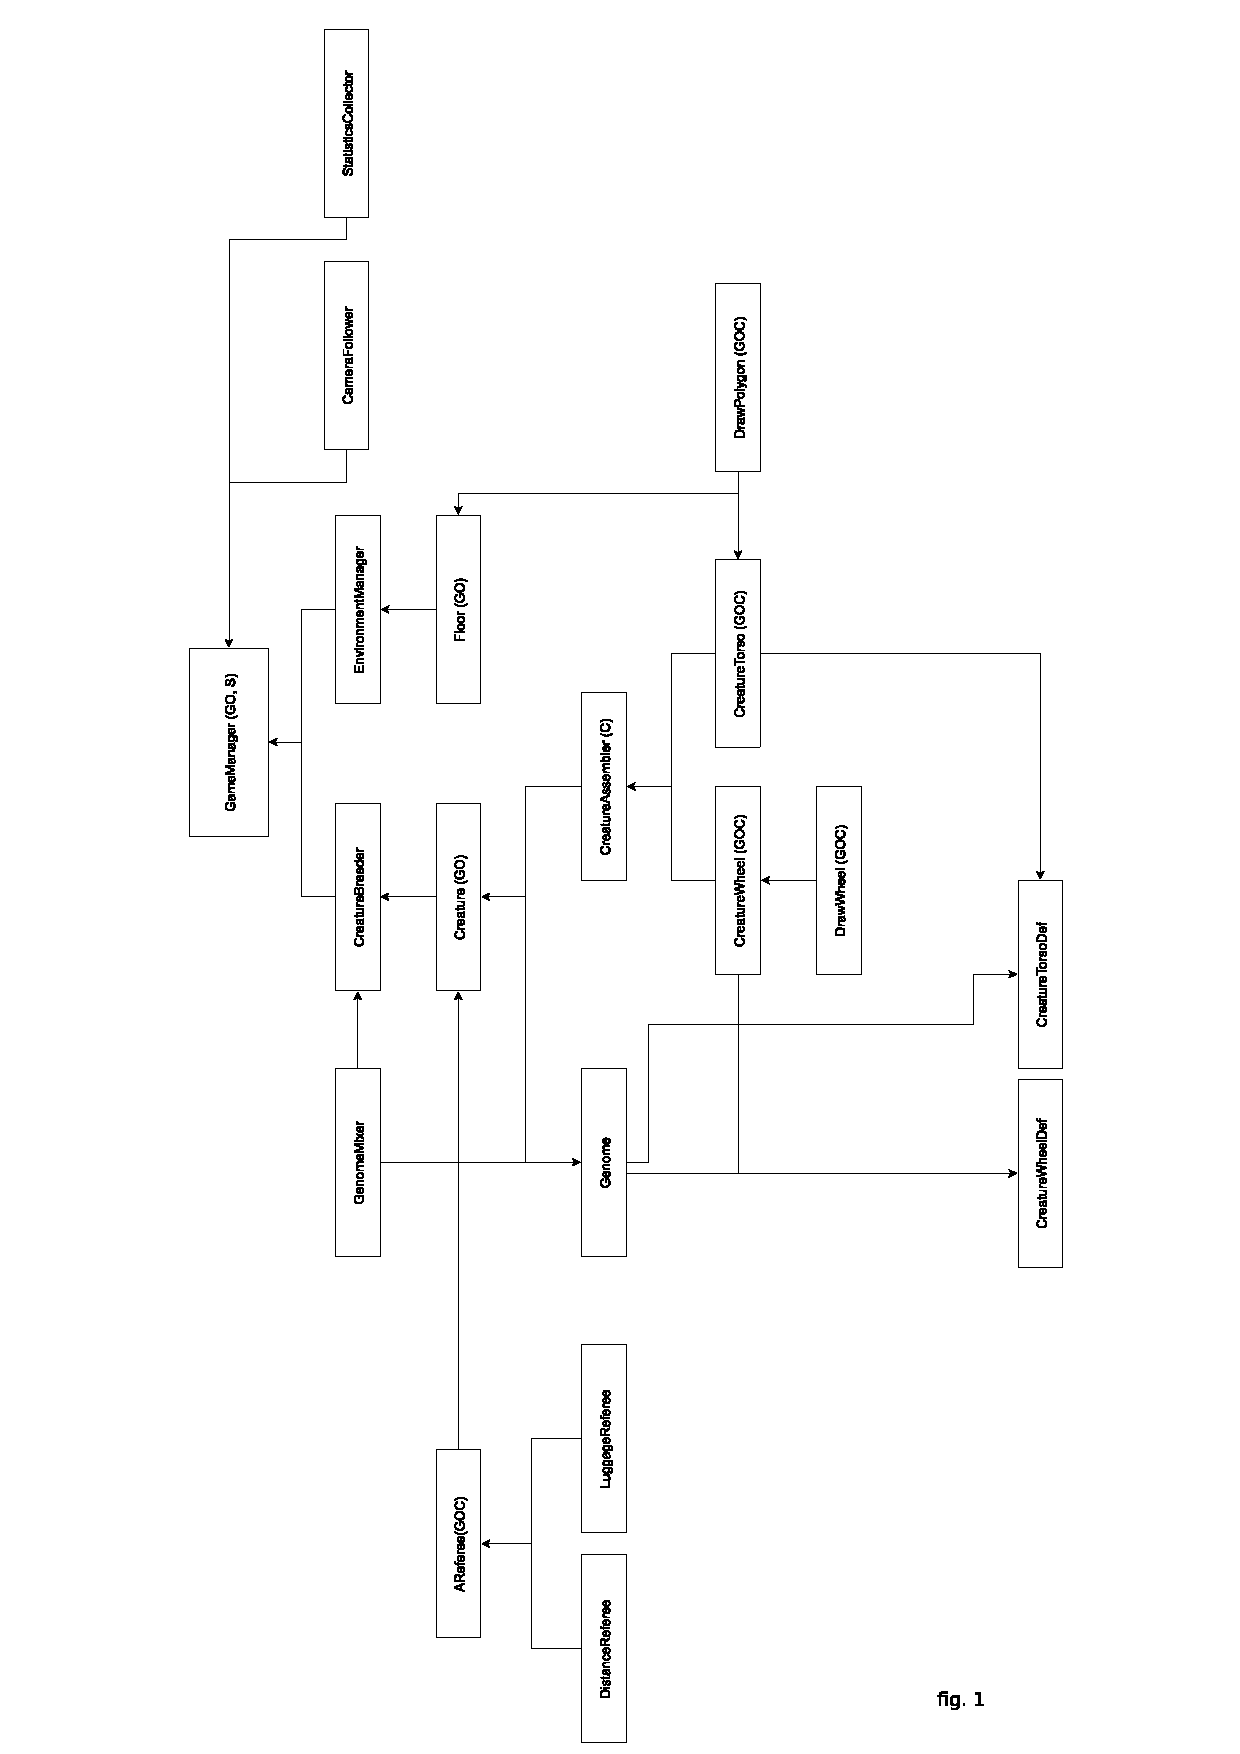
\includepdf[pages=-]{uml.pdf}
\end{document}
